\documentclass[man, floatsintext]{apa7}

\usepackage[american]{babel}
\usepackage{amsmath}
% \usepackage{apacite}

\usepackage{csquotes}
\usepackage[style=apa,sortcites=true,sorting=nyt]{biblatex}
% \DeclareLanguageMapping{american}{american-apa}

\addbibresource{bibliography.bib}

\title{The structure of developmental variation in early childhood}
\shorttitle{Structure of developmental variation}

\author{\vspace{1em}}
\affiliation{\vspace{1em}}
% \authorsnames{Ben Stenhaug, Nilam Ram, Michael C. Frank}
% \authorsaffiliations{Stanford University}

% \leftheader{Stenhaug}

\abstract{Do children's abilities develop in tandem or surge on their own? Piaget proposed that development proceeded globally through
stages; more recent theories view development as more modular. The developmental differentiation hypothesis suggests that the structure of a child's development is unitary in infancy but becomes more complex with age. We investigate this hypothesis using two large datasets of parent-reported developmental milestones (in Mexican children, N=2023, and in international users of a mobile app, N=1800). Applying item response theory models, we find that variation in development across infancy and early childhood is multidimensional. Consistent with the differentiation hypothesis, differences among older children are better described by higher-dimensional models; and within-person changes in underlying abilities that are highly coupled early in life become less coupled over the first 18 months of life.  Our work provides a model-based method for answering basic theoretical questions about the nature of change in childhood.}

\keywords{child development, differentiation, milestones, item response theory, model comparison }

% \authornote{We thank Kinedu, Inc.~for financial support and data sharing and
% George Kachergis, Alex Carstensen, Ben Domingue, and Ann Weber for
% comments on early versions of this paper. The research reported here was
% also supported by the Institute of Education Sciences, U.S. Department of
% Education, through Grant R305B140009 to the Board of Trustees of the
% Leland Stanford Junior University. All authors contributed to research design and paper writing. MCF obtained data. BS wrote code. Correspondence concerning this article should be addressed to Michael C. Frank, Department of Psychology, Stanford University, 450 Jane Stanford Way, Stanford, CA 94305, USA. E-mail: mcfrank@stanford.edu}

% % Please add here a significance statement to explain the relevance of your work
% \significancestatement{How do children vary? Do some children develop globally faster or slower than others, or is variation more discrete (e.g., in motor or language skill)? Variation between children has
% often been assumed to be unifactorial or multifactorial without formal
% evaluation. Our work here uses psychometric modeling and big-data
% approaches to evaluate this dimensionality empirically. We find evidence for multidimensionality, and further evidence that this dimensionality increases with age. This work implies that measures of developmental variation should move
% beyond assumptions that differences and progression of children's
% development can be represented as a homogenous process, and toward
% multi-dimensional representations of within-person change.}


% \authorcontributions{}

% \authordeclaration{The authors declare no conflicts of interest.}


% \correspondingauthor{\textsuperscript{1} To whom correspondence should
% be addressed. E-mail:
% \href{mailto:benastenhaug@gmail.com}{\nolinkurl{benastenhaug@gmail.com}}}

% Keywords are not mandatory, but authors are strongly encouraged to provide them. If provided, please include two to five keywords, separated by the pipe symbol, e.g:
%  \keywords{   }


\begin{document}

\maketitle

How do young children grow and change? Is child development a single
unified process or a multitude of processes that carry their own
constraints and timescales? Piaget famously proposed a stage theory in
which many seemingly distinct mental processes developed in concert
through a common set of operational stages \parencite{flavell1963}. In contrast, modern
theories propose that there are different facets of children's mental
life and that these facets each develop on their own timetable \parencite{gelman1983}. And attesting to a folk theory of developmental multi-dimensionality, the
grandmother of one author was known to assert that
``children either walk early or else they talk early.''

A theoretical and practical understanding of how children grow and change
provides the underpinning for parents', teachers', and health professionals'
efforts to observe and facilitate children's development. However, the process of assessing
children's developmental status critically depends on our assumptions
about the structure of developmental change -- in particular, whether
there is a single unified process that can be measured through tracking
of developmental milestones. Global assessment of developmental status
via a series of binary milestones (e.g., ``Can your child walk at least
ten steps unassisted?'') is both a standard feature of pediatrician
visits and a gold standard for assessing children's developmental
status in the research and intervention communities \parencite{sheldrick2019,bayley2009,bricker1999,mccoy2019,weber2019}. In such
assessments, which are typically but not always conducted via parent
report, most
instruments assume a unifactorial model \parencite[although some also
provide subscale scores;][]{bayley2009} in which developmental progress is often treated as an
amalgam of motoric, cognitive, and language achievements.

Further, the dimensionality of children's variation is not necessarily constant -- it could itself change developmentally.
Indeed, some early work argued that a single, general
ability factor transitions into multiple factors between 8 and 18 years of age
\parencite{garrett1946}. We refer to the general idea of an increase in the factor structure of developmental variation as ``the differentiation hypothesis.'' The differentiation hypothesis was later extended to the
differentiation-dedifferentiation hypothesis, which holds that abilities
separate during the first half of the life span and then collapse back
together later in life \parencite{lienert1964,tucker-drob2009,breit2020}. Being a within-person hypothesis, the
strongest evidence for the (de)differentiation hypothesis requires
longitudinal data so as to identify the expanding or collapsing of
factors within individuals \parencite{hulur2015}.

To our knowledge, no prior studies have tested the differentiation hypothesis from birth through early childhood. There is mixed evidence of differentiation in middle childhood and adolescence \parencite[e.g.,][]{juan-espinosa2006,shing2010,breit2020}
and mixed evidence of de-differentiation in adulthood \parencite[e.g.,][]{hartung2018,li2004} -- see \cite{breit2021} for review -- but most of these studies have used standardized measures of intelligence (and various subtests) as their primary measurements, rather than taking a holistic view of development. Perhaps for reasons of measurement and data availability, nearly all studies begin at school age \parencite[see][table 2]{breit2021}. Finally, neither the differentiation hypothesis nor de-differentiation hypothesis are typically evaluated from a  within-person perspective \parencite[see][as an exception]{hulur2015}.

Although large-scale datasets are everywhere \parencite{tsai2015}, few
focus on early childhood \parencite[cf.][]{mindell2016,milne-ives2020}.  Those that do include infants and young children typically focus on a single aspect of development, like sleep \parencite{mindell2016} or language \parencite{frank2021}. Comprehensive empirical
examinations require longitudinal data that tracks how many children
progress through many milestones, with limited missingness and
reasonably short intervals between assessments. Although data quality often remains a
challenge \parencite{milne-ives2020}, the big-data obtained
via mobile apps open new opportunities for studying how development
manifests in real-world settings.

This paper leverages two datasets -- survey data and mobile app data, both provided by parents as their children developed -- to explore
the structure of developmental variation in early childhood. In the
cross-sectional survey data, middle-class Mexican parents of children
between 2 and 55 months old (N = 1,946) provided comprehensive reports
about whether or not their children had achieved 414 developmental
milestones. In the longitudinal mobile app data, over 20,000 parents
repeatedly reported on their child's achievement of collections of
age-specific developmental milestones as part of their use of a mobile
application that provided child development related video content. The
app used milestone reports as a method for assessing children's progress
and serving appropriate content. By using survey data in conjunction
with app data, we leverage the structure of each data source to provide
empirical information about the structure of developmental variation
in early childhood.

The foundations of our inquiry are built from  principles of
measurement/testing and computational data science. We use psychometric
models to instantiate specific hypotheses about the structure of children's development
and to assess how well various structures fit the data. In particular, we
leverage item response theory (IRT) models \parencite[first developed by
Educational Testing Service to measure students' academic performance;][]{lord1980}, to describe the structure of developmental variation in early
childhood. We also leverage the sheer size of these newly available data
through use of cross-validation and construction of hold-out data sets
that facilitate iterative exploration and confirmation of the structural
and differentiation hypotheses. In doing so, we propel forward the
integration of developmental and data science now afforded by the
arrival and curation of big data from the deployment of mobile technologies.

We conducted two studies using these datasets. Study 1 used a series
of item response models with different numbers of factors to describe
the structure of between-child developmental variation in the survey
data.
% As evidence for multidimensionality, we found that models with
% more factors performed better according to out-of-sample accuracy. And,
% consistent with the differentiation hypothesis, models with more factors
% provided more complete descriptions of the differences among older
% children.
At its core, the differentiation hypothesis is a theory about how
individual children develop, however. In particular, the differentiation
hypothesis posits that within-child covariation between underlying ability
factors will be high very early in life and decrease as children age.
Between-child differences, like those examined in Study 1, are often
examined in relation to the age-related differentiation hypothesis, but
risk falling prey to the ecological fallacy: seeming age differences in structure might
instead indicate differences in developmental timing or selection. Thus,
in Study 2, we leveraged additional longitudinal data that more
specifically supports examination of how the covariance between
developmental factors changes \emph{within-person} over time.
% Specifically, using a 2-factor model from Study 1 -- where the 1st factor
% serves as a broad indicator of physical achievement and the 2nd factor
% serves as a broad indicator of linguistic achieve -- we model both how
% children develop over time and how the coupling between gains on each of
% the two factors changes with age. Here,
% We find strong evidence for the
% within-person differentiation hypothesis, with the high early
% covariation between the two factors systematically decreasing across
% early childhood.


\section{Open Practices}

All data and code necessary to reproduce our results are publicly available at \url{https://osf.io/5426p/?view_only=12520097ba674ab1923b9f0738e37354}.\footnote{We also include in this repository a preregistration of followup analysis of a different dataset. We report on these data in our Supplemental Information and explain why we eventually deemed the dataset unsuitable for our analysis.}

% . We deviated from this preregistration for two reasons. First, we had not planned to use longitudinal data reported in Study 2 but came to appreciate the importance of these data for examination of differentiation as a within-person phenomenon. Second, we had failed to appreciate the degree to which lack of milestone
% overlap across ages (i.e., planned missingness for older children to
% younger milestones and vice versa) jeopardized our ability to make valid cross-age
% comparisons. }
%
\section{Study 1}

% As children develop, they achieve -- and sometimes move through -- many milestones,
% including shaking objects, crawling, pointing, taking turns, and drawing
% shapes.

While developing and norming a set of web- and smartphone-based
parenting applications, Kinedu, Inc. obtained data on whether many
children of different ages had achieved a wide variety of developmental milestones. In Study 1, we use these data to assess the latent dimensionality of developmental variation and provide a first test of the differentiation hypothesis.

\subsection{Methods}

\subsubsection{Survey Data}

Surveys were completed by
middle- and upper-class Mexican parents whose children were in group
care. Each parent reported on whether or not
their child had achieved each of 414 milestones, including 180
physical milestones (e.g., child can go from sitting to kneeling), 100
cognitive milestones (e.g., child can find objects on the floor), 75
linguistic milestones (e.g., child can say four words), and 59
social-emotional milestones (e.g., child shows concern for a crying
friend). Complete data with no missing responses for all 414 milestones we available for 2,023 children. After removing reports about children < age 2 months due to concerns about data quality (e.g., 40\% of 0- and 1-month-olds had surprisingly achieved at least 80
milestones), the final analysis data included reports about 1,946 children age 2 to 55
months achievement of 414 cognitive, linguistic, physical and
social-emotional milestones. As shown in Figure \ref{fig:partage}, number of milestones achieved increased with age, with most
children having achieved about 50 of the developmental milestones by age 1 month, and about 300 of the developmental milestones by age 24 months.


\subsubsection{Data Analysis}

Our examination of the dimensionality of children's achievement of developmental milestones  and the differentiation hypothesis uses an exploratory, iterative model building approach.

\paragraph{Item response models}

Parents' survey reports were binary responses indicating whether a child has not or has achieved 414 behaviors that are more or less difficult. These data have the same structure as item response data commonly obtained in educational settings where, for example, the standardized test instruments used to track students' achievement and learning consist of students' responses to long batteries of items that are graded as correct or incorrect. Item response models provide a robust framework for assessing the factorial structure of such instruments, the relative difficulty of each item in the instrument, and respondents' level of performance on the abilities or latent factors measured by the instrument. Here, we leverage these models to assess and describe the structure of children's achievement of developmental milestones.

Parents' survey responses were modeled using a series of standard two-parameter logistic (2PL) item response model. Specifically, the probability of child $i$, $i = 1, \ldots, I$, having achieved developmental milestone $j$, $j = 1, \ldots, J$, is \begin{equation}\label{eq:irt}
P(y_{ij} = 1 | \boldsymbol{\theta_i}, \boldsymbol{a_j}, b_j) = \sigma(\boldsymbol{a}_{j}^{\top}\boldsymbol{\theta_i} + b_j)
\end{equation} where $\boldsymbol{\theta}_{i}=(\theta_1, \dots, \theta_m)$ indicates the $i$th child's level of ability on each of $m$ latent factors, $\sigma(x) = \frac{e^x}{e^x + 1}$ is the standard logistic function, and $b_j$ and $a_j$ indicate the relative easiness/difficulty (i.e.~intercept) and discrimination (i.e.~slope; factor loading) of each item/milestone.
We explored the factor structure of children's developmental achievements by fitting five 2PL models with $m = 1, \ m = 2, \ m = 3, \ m = 4$ and $m = 5$ latent factors (20), referred to hereafter as the 1F, 2F, 3F, 4F and 5F models.


\paragraph{Baseline model}
A baseline (non-item response) developmental model was constructed where probability of child $i$ having achieved developmental milestone $j$ is a simple function of child's age (in
months), specifically the modal response for a particular milestone at a given age. For example, parents report that 64\% of children age 16-months can identify animals by their sounds; the baseline model assumes that all 16-month-olds have achieved this milestone. This baseline model thus provides a developmentally aware data-driven index of predictive performance that might be surpassed by item response models with different numbers of latent factors.

\paragraph{Model comparison}

The dimensionality of children's achievement of developmental milestones and the differentiation hypothesis were examined through formal comparison of the five 2PL item response models and the baseline model across the entire age span as well as across 5 age groups. Although model comparison in IRT is typically based on information criterion such as AIC and BIC \parencite{maydeu-olivares2013}, the comparisons are less accurate when working with modest sample sizes or when models are misspecified \parencite{mcdonald1995}. We avoided these potential errors in dimensionality identification through use of the cross-validation approaches commonly used in data science, and that have been adapted for use with item response models \parencite{bergner2012}.

Cross-validation was done across 8 folds. The data were partitioned into 8 folds using a stratified randomization procedure whereby each child's data was split into and treated as data from 8 ``sub-children'' and each fold contained data from exactly one of these sub-children. Following typical practice, model fitting and assessment was done by repeatedly circulating through 7 in-sample folds and 1 out-of-sample fold. At each step we fit the baseline and 1F to 5F models to the in-sample data. The item response models were estimated using marginal maximum likelihood estimation (MMLE; which estimates milestone parameters but not child parameters \parencite{baker2004}), using the standard EM algorithm \parencite{bock1981} for models 1F and 2F, and using quasi-Monte Carlo EM \parencite{jank2005} for models 3F to 5F. In all relevant models, milestone parameters were estimated under an oblimin rotation that allowed the factors to correlate \parencite{jennrich1966}, without priors on $a_j$ (so as to not
interfere with interpretations of dimensionality) and with a Normal(0,3) prior on all $b_j$ values (for stabilization). After the model parameters were obtained, we estimated factor scores using expected a posterior (EAP) with an m-dimensional normal prior, as calculated by Gauss-Hermite quadrature \parencite{embretson2013}, and used the item parameters and estimated factor scores to predict the probability of each of the out-of-sample milestone responses, and classifying the prediction as correct when the predicted probability was greater than 50\% and the milestone was achieved or when the predicted probability was less than 50\% and the
milestone was not achieved).

\paragraph{Estimating the relationship between age and dimensionality}

The differentiation hypothesis -- the relation between dimensionality and age -- was examined by quantifying the relative gain of the higher dimensional (2F to 5F) models over the 1F model.Intuitively, gain is the percent of possible improvement in accuracy of the higher dimensional model over the 1F model. More specifically,
where $\text{acc}_\text{model}$ is the out-of-sample accuracy from a
higher-dimensional model and $\text{acc}_\text{1F}$ is the
out-of-sample accuracy of the 1F model, gain is calculated as
$\frac{\text{acc}_\text{model} - \text{acc}_\text{1F}}{1 - \text{acc}_\text{1F}}$.
First, we examined each model's \emph{performance} by calculating gain for four age-group partitions, each covering roughly 1-year age groups: age 2 to 11 months, 12 to 23 months, 24 to 35 months, and 36 to 47 months and 48 to 55 months, with the upper two age groups consolidated together to obtain similar sample size in each group. This examination involved estimating 40 models (5 models $\cdot$ 8 folds). Second, acknowledging that the structure of developmental variation might change with age, we estimated each model separately for each of the four age groups. This involved estimating 160 models
(5 models $\cdot$ 8 folds $\cdot$ 4 age groups) and calculating gain for each model in each age group partition. Notably, in this scenario, there are cases where nearly all (or no) children in a particular age group have accomplished specific milestones (e.g., all older children being able to say four words). To prevent this kind of homogeneity from destabilizing model estimation, milestones were filtered from the age group-specific data when more than 97.5\% or fewer than 2.5\% of children had achieved that milestone. Results from the full set of model comparisons informed evaluation of the differentiation hypothesis.
% Figure \ref{fig:study1} shows results from both techniques,
% with the top panel corresponding to the first and the bottom panel
% corresponding to the second.

\subsection{Results}

\begin{figure}
\centering
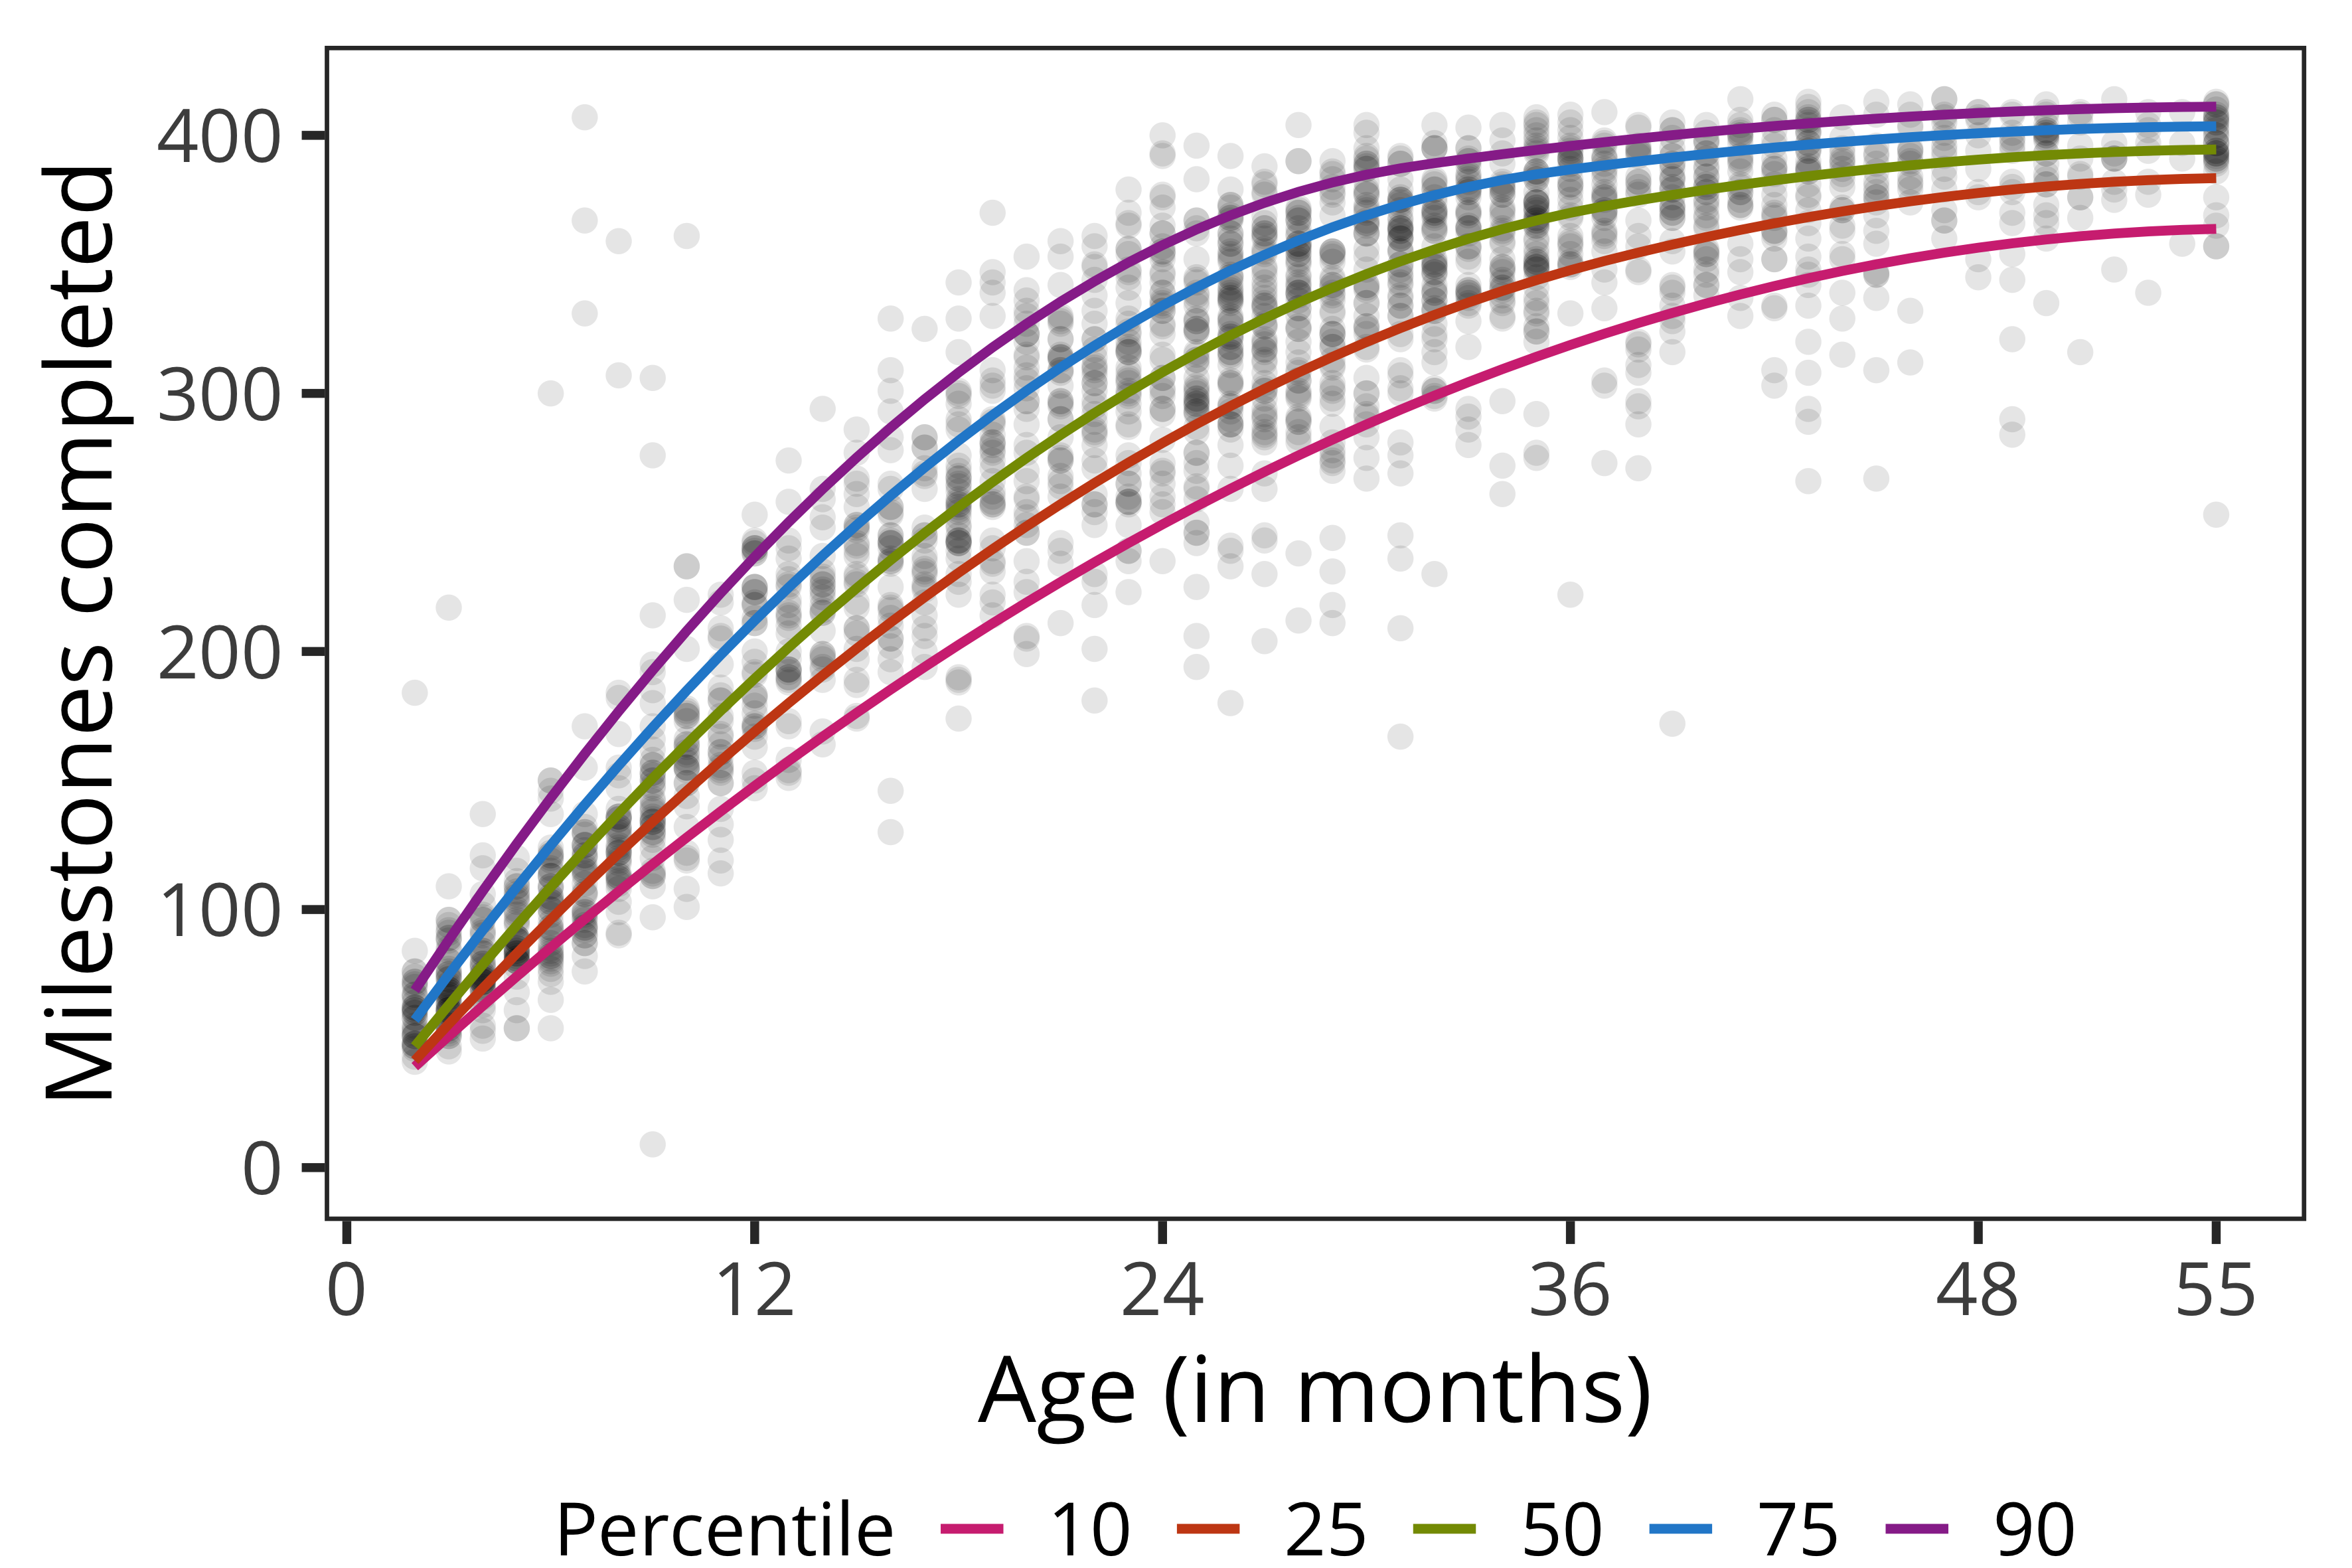
\includegraphics[width=4in]{figures/01_achieve_by_age.png}
\caption{Number of the 414 milestones completed by age with percentile curves; data are from the survey reported in Study 1. Points represent individual children.}
\label{fig:partage}
\end{figure}

\subsubsection{Developmental Variation is
Multidimensional}\label{developmental-variation-is-multidimensional}

Results from fitting the baseline and five 2PL item response models are shown
in Table \ref{tab:study1results}. Baseline performance was very strong (86.9\%), suggesting that a substantial amount of variation is related to children's age, confirming the developmental nature of the data and inquiry. While the unidimensional model (1F:
88.8\% accuracy) had better performance than the baseline model, the
multidimensional models (2F to 5F) all performed even better
(\textgreater{} 89.3\%). The 5F model provided 89.8\% out-of-sample
accuracy, and thus (of the models fit) provided the best predictive
performance. Gains over the baseline model were relatively small in absolute terms, in part because age is such a strong predictor and in part because the data include measurement error that imposes a predictive ceiling. Differences between models are slightly clearer when examining the proportion of total variation explained. Here, the 4F model shows substantial (14\%) improvement over the 1F model. Notably, the 5F model explained less variance than the 4F model, indicating that further increases in dimensionality would not provide better fit.

Each of the models revealed a consistent structure, where the 1st factor is characterized by high discrimination parameters (i.e., factor loadings) for linguistic milestones (i.e., linguistic milestone discriminate well between children high and low on the 1st factor; Figure \ref{fig:discs}), and, in models 2F to 5F, the 2nd factor is characterized by high discrimination parameters for physical milestones. In models 3F to 5F, the 3rd, 4th and 5th factors are characterized by discrimination parameters that are relatively close to zero, indicating that these factors indicate a mix of types of milestones.

\begin{table}[!ht]
\caption{\label{tab:study1results}Model performance as measured by out-of-sample accuracy. Higher-dimensional models perform better.}
\centering
% \fontsize{8}{10}\selectfont
\begin{tabular}[t]{lcc}
\toprule
Model & Out-of-sample Accuracy & Proportion of Variance\\
\midrule
5F & 89.8\% & 73.0\% \\
4F & 89.7\% & 74.5\% \\
3F & 89.5\% & 73.3\% \\
2F & 89.3\% & 66.1\% \\
1F & 88.8\% & 60.1\% \\
Baseline & 86.9\% & - \\
\bottomrule
\end{tabular}
\end{table}

\begin{figure}
\centering
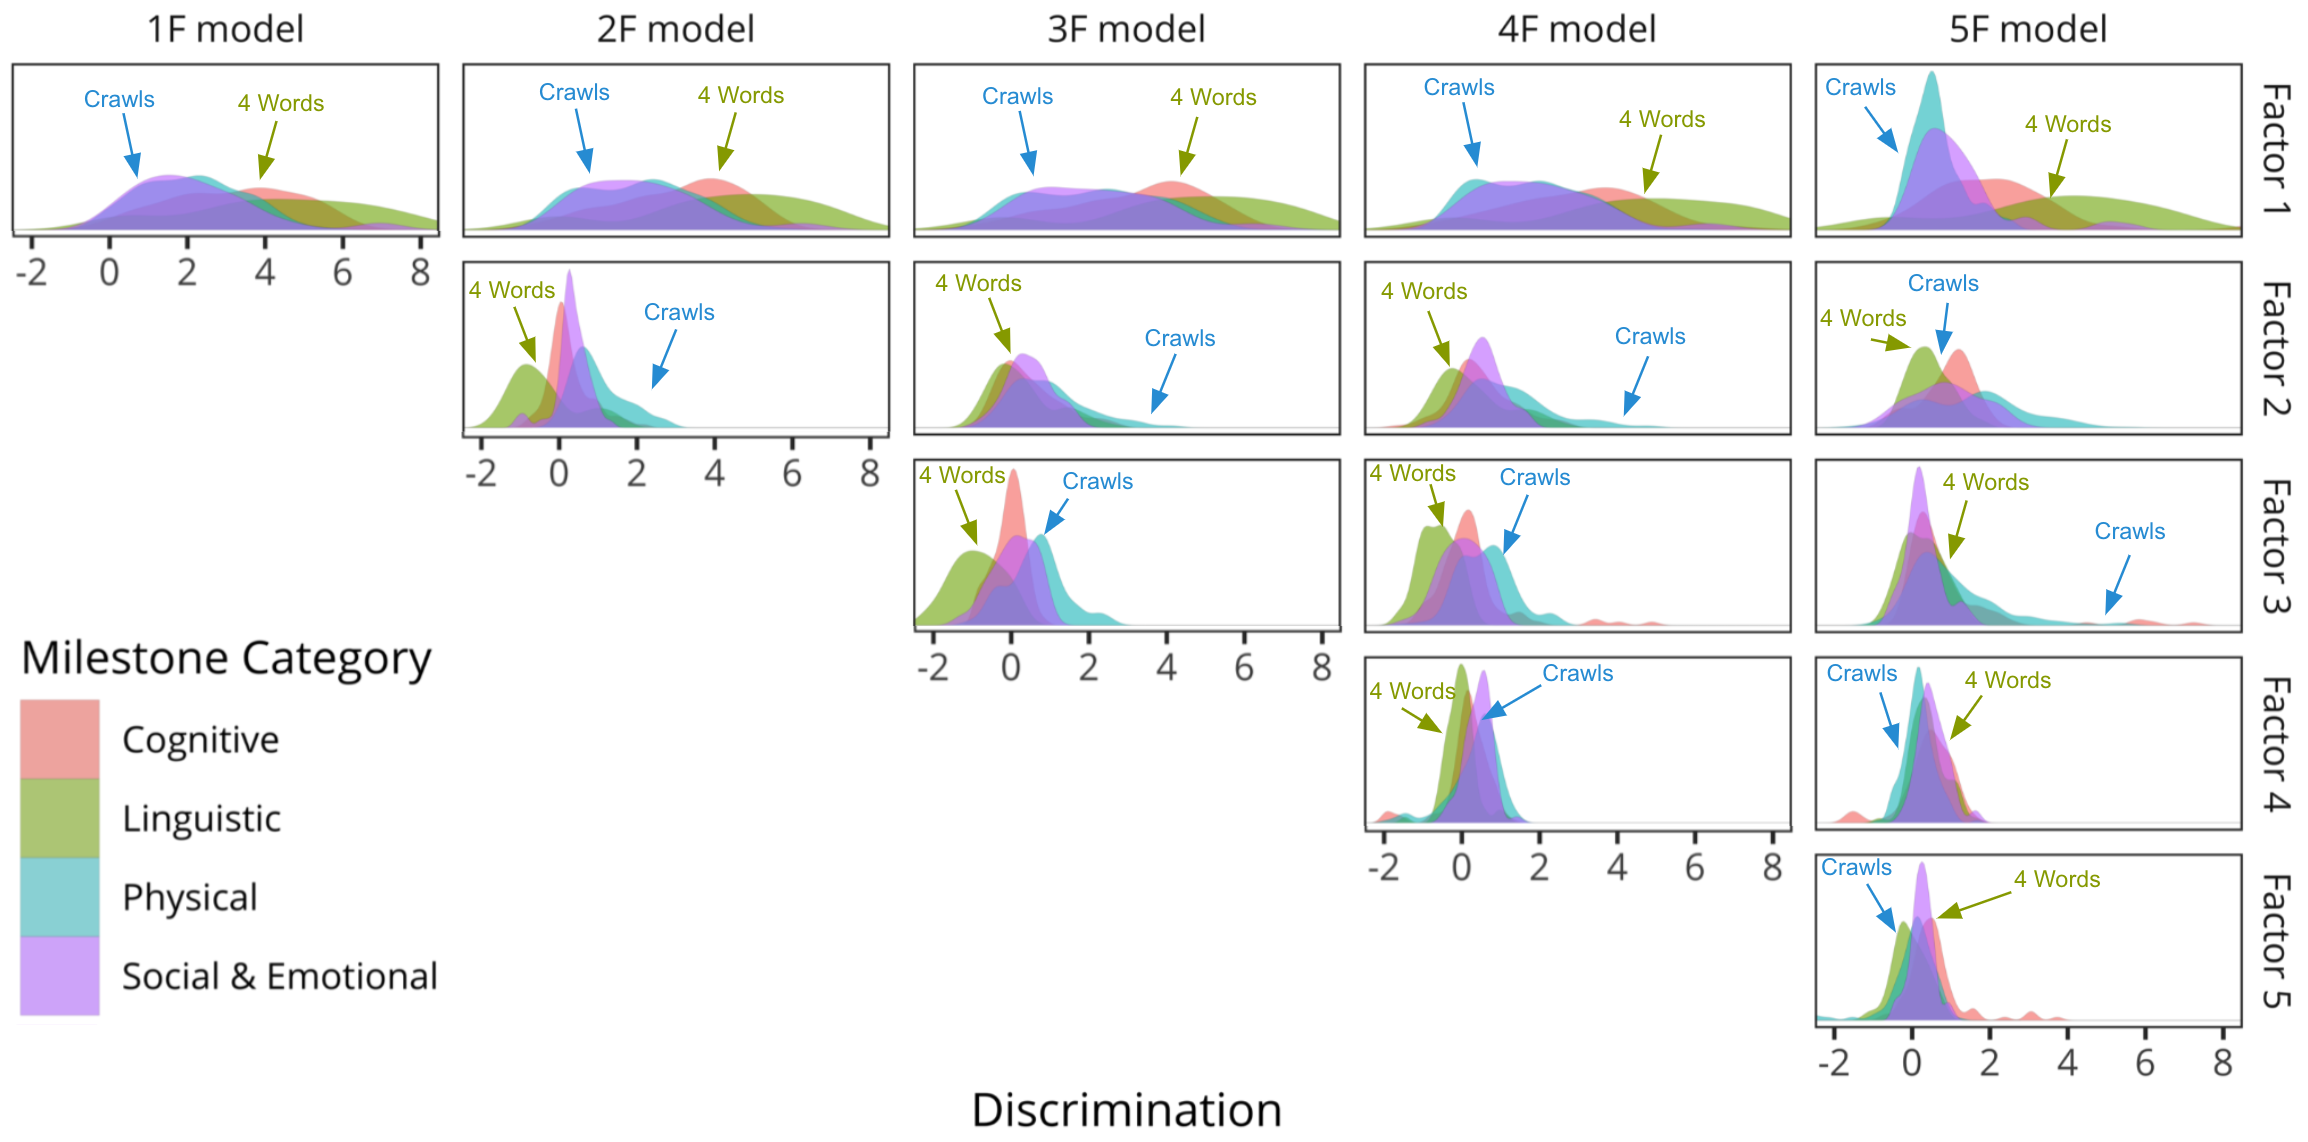
\includegraphics[width=\columnwidth]{figures/models_new.png}
\caption{Distribution of discrimination parameters for the factors of the 1F, 2F, 3F, 4F, and 5F models. Columns of subplots show models, rows show factors, and distributions are the density of discrimination parameter estimates, colored by broad milestone categories. In each of the models, linguistic milestones load heavily on the 1st factor. Additional factors tend to be composed of other milestone categories—for example, physical milestones tend to load heavily on the 2nd factor. As expected, the typical discrimination decreases for later factors. Arrows track the location of two milestones, crawling (physical) and saying at least 4 words (linguistic), across each of the factors.}
\label{fig:discs}
\end{figure}

\subsubsection{Older Children's Milestones are More Accurately Described
by Higher-Dimensional
Models}

The between-person version of the differentiation
hypothesis suggests that the abilities of older children are better described by models with
higher-dimensional structure. Gain of the 2F to 5F models over the 1F model (distance between the 1F model's performance and 100\% that the model achieves) in each of the age-group partitions is shown in the top panel of Figure \ref{fig:study1}. For example, for
24 to 35-month-olds, the 5F model has 88.4\% accuracy as compared to the
1F model which has 87.2\% accuracy. The gain of the 5F model over the 1F
model is thus $\frac{88.4\% - 87.2\%}{100\% - 87.2\%} = 9.4\%$. The lines indicate that the 5F model performs best for each bin and also performs particularly well for the older age
groups. The relative increase in gain for the 5F model (and other multi-dimensional models) at older ages is consistent with the differentiation hypothesis.


\subsubsection{Differences Between Old Children Are Better Described by
Higher-Dimensional
Models}

Leveraging the sheer size of the data to push beyond evaluation of predictive performance of global models in different age groups, we also examined relative performance within each age-group partition separately. In particular, we conducted the 8-fold cross-validation procedure again within each age-group partition of the data. The bottom panel of Figure \ref{fig:study1} shows the gain for
each of the higher dimensional models over the 1F model for each age
group fit separately. The relative gains of the higher dimensional age-specific models provide similar but perhaps somewhat stronger evidence for the differentiation hypothesis: The gain of higher dimensional
models is modest for the youngest age group and substantially higher for
older age groups.

\begin{figure}[t]
\centering
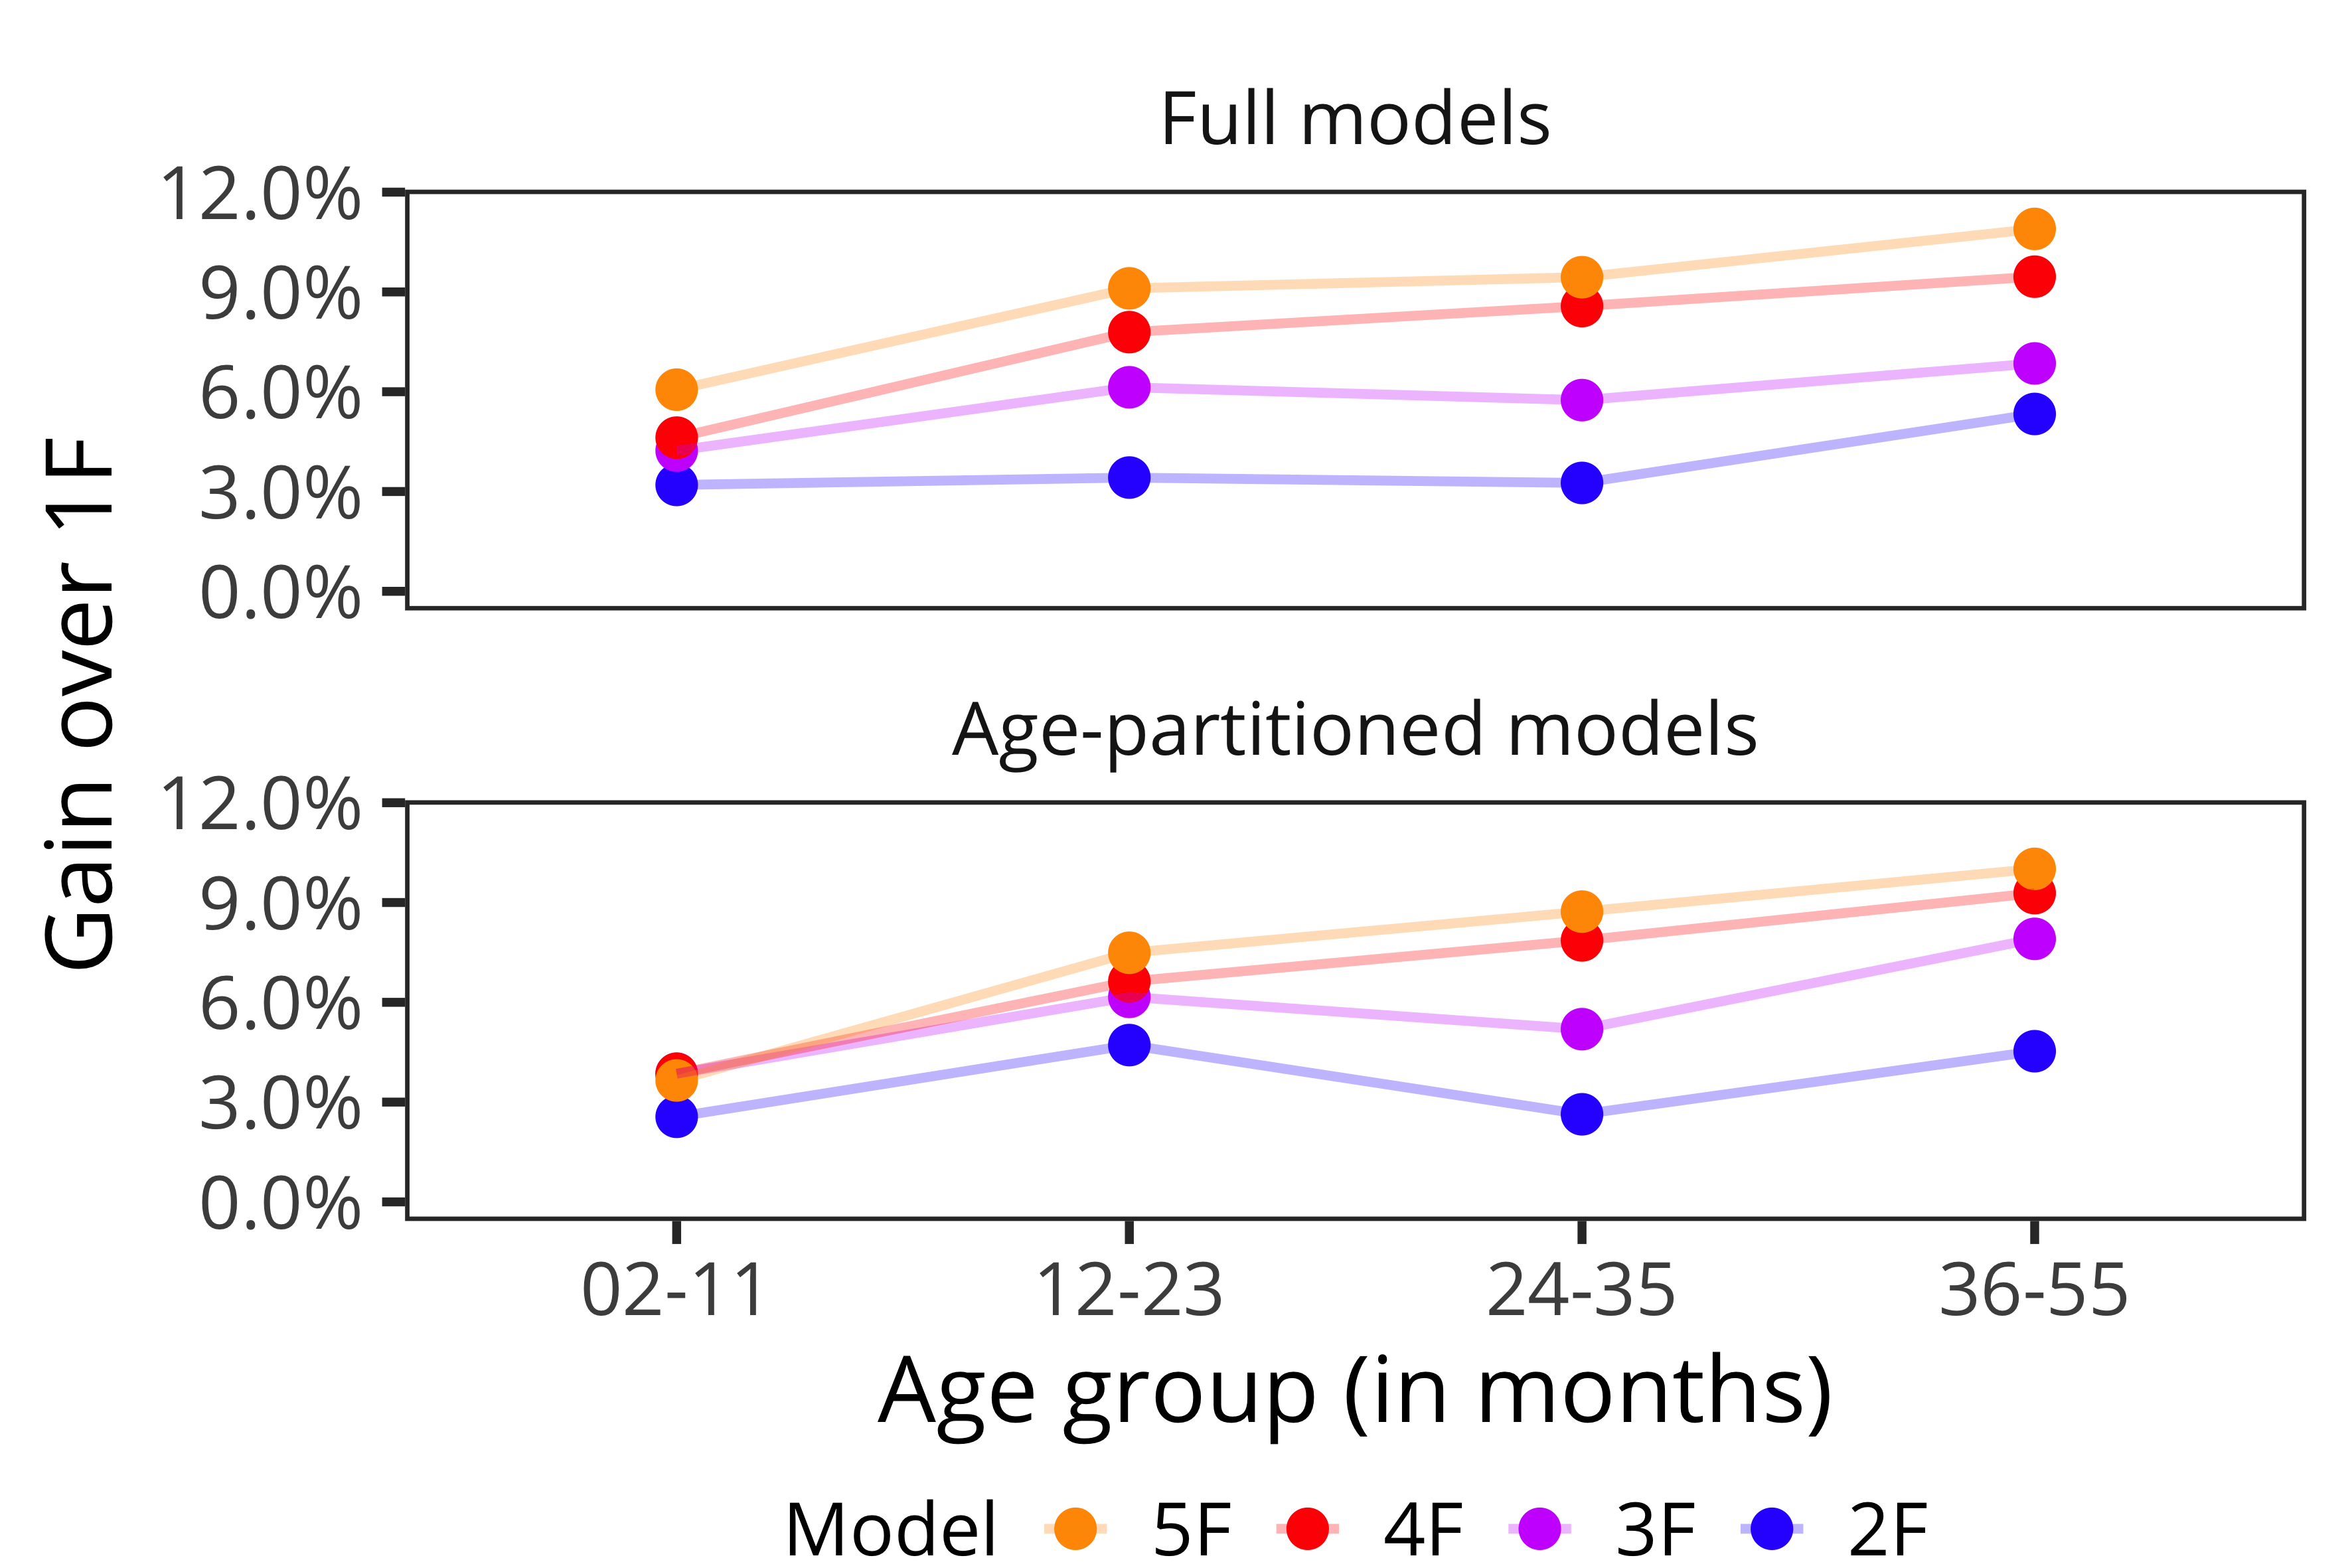
\includegraphics[width=5in]{figures/study1.png}
\caption{Gain of higher-dimensional models over 1F model. Gain is defined as the proportion of the distance between the 1F model’s performance and 100\% that the model achieves. Top panel shows models fit to the full dataset but evaluated on each age partition, bottom panel shows models fit separately to each age partition.
% The top panel shows that when each model is fit to the full dataset, higher-dimensional models perform particularly well for older age groups. The bottom panel shows that when each model is fit separately to each age group, higher-dimensional models perform particularly well for older age groups.
}
\label{fig:study1}
\end{figure}



\section{Study 2}

%
% The results from Study 1 suggest that children's development is multidimensional and provide compelling support for the differentiation hypothesis.
Drawing inferences about within-child, developmental processes from cross-sectional, between-child data runs the risk of committing a version of the ecological fallacy \parencite{piantadosi1988}. Here, the risk is that patterns observed in the differences between children are not necessarily indicative of the patterns that manifest within-children across time.
% Additionally robust assessment of the differentiation hypothesis requires analysis of longitudinal data.
The differentiation hypothesis suggests that the structure of children's
abilities expands with age. That is, the extent to which underlying abilities are ``coupled'' should decrease with age.

Prior to differentiation, age-specific deviations from a child's developmental trajectory in one underlying ability should be tightly coupled to to age-specific deviations in other underlying abilities. For example, when a child surges ahead on motor ability in a particular month, they will also surge ahead on linguistic ability. If there is differentiation, the extent of coupling should decrease with age, such that surges in motor ability will be less or not at all coupled with changes in linguistic ability. To test this hypothesis in Study 2, we use data from the Kinedu mobile app, taking advantage of parents' longitudinal reporting of milestone data.
% we adapt methods developed in
% examination of dedifferentiation of cognitive abilities in old age \parencite{hulur2015}
% to analysis of factor scores obtained from multidimensional item
% response models. Our dataseti of the milestone data obtained on up to 21 occasions as
% children moved through early childhood.
%
% As detailed below, we use multilevel model models of change to examine if and how age moderates
% the extent of within-person coupling in the occasion-to-occasion changes
% in factors underlying milestone achievement (estimated using item
% response models), after controlling for individuals' general
% developmental gains. Our expectation is that, separate from the
% long-term developmental trends, within-person variations on 2 underlying
% ability factors will be tightly coupled (i.e., dedifferentiated) at
% earlier ages and that the extent of coupling will decrease towards zero
% as children get older and the underlying factors differentiate.


% Computing coupling of this type involves five distinct steps (Figure
% \ref{fig:study2} visualizes the first four). The first step was to develop an
% appropriate measurement model. Because the survey data is complete and
% likely to be higher quality, we chose to use the survey data to develop
% this model. To ensure that the model was well-calibrated for the app
% data, we filtered to children 24 months of age or younger and removed a
% small number of children with an unexpected number of milestones
% complete for their age (e.g., a 9-month-old with more than 350
% milestones complete). A 2F model offers good fit and an interpretable
% factor structure for this population. The 1st and 2nd factors capture 35\% and
% 20\% of the survey data variance, respectively (an additional factor
% would explain only 5\% more variance). These factors appear to load more heavily on physical milestones vs. linguistic milestones, respectively.

% % The logic of our method is based on
% % viations from a child's developmental pathway.

% The second step was to estimate factor scores for each
% child-timepoint in the app data according to the parsimonious 2F model
% fit to the survey data. As expected, these factor scores are highly
% correlated with age. In the third step, we separately estimated a
% quadratic developmental pathway for each child. In the fourth step, we
% calculate the deviation from the child's developmental pathway for each
% timepoint.


% The fifth and final step was to fit a mixed-effects model to estimate
% coupling across the age span for all children. The model predicts the deviation for one factors using the other factor's deviation (and interactions with age), while controlling for differences between individual children using random effects (following 10). Larger coefficients on factor deviation indicate greater coupling, such that, for example, if at a particular time point the child increases on factor 1 they are more likely to increase on factor 2.



\subsection{Methods}

\subsubsection{App Data}

Longitudinal data were sourced from Kinedu, Inc.'s mobile application. As part of using the app, parents of children were asked to
respond to 20-50 milestones about their child every few months. Country of residence for parents was unknown but the vast majority of users came from the United States, Mexico, and Brazil. As with
many mobile apps, usage is non-uniform, such that many users use the app
once or only occasionally, while a smaller number of users use the app frequently.

% We focus here on the most frequent users of the app, as their relatively dense data provide the best opportunity to test hypotheses about within-child change. We
% selected data from children with at least 6 timepoints, where a
% timepoint contains at least 5 responses to each of the 4 milestone
% categories. We also focus here on children between 2 and 18 months old
% because parents typically use the app when their child is in this age
% range and so there were few children with dense data in older age ranges.

Our analysis of within-child coupling of abilities makes use of data collected between
when the set of 414 milestones used in Study 1 was first introduced (12/01/2017) and the start
of our data analysis (12/16/2020). After collecting reports that parents provided about their children's achievements within 5-day windows together into a single record, we filtered the data down to those records that included at least 5
responses within each of four milestone categories (cognitive, linguistic, physical,
social-emotional), minimum of 20 milestones. We focused on reports provided by parents who reported on their child at least 6 times when the child was between ages 2 months and 18 months. This subsetting effectively mitigated any floor or ceiling effects while also reducing any potential selection bias introduced by parents who use the app inconsistently or elect to use the app only when the perceive their child is exhibiting atypical development.

The remaining data consisted of 177,934 reports about 21,861 unique children. Leveraging big-data and open-science principles, we randomly drew data for three independent N = 600 samples (total of 1,800 children). The first "exploratory" sample was used when developing the methods and models. The second and third ``replication'' samples were used to test the validity of the results obtained with the exploratory sample. The data thus facilitate initial inductive exploratory modeling, deductive confirmatory modeling, and future replication and extension - and set a new standard for how such data are used and shared.


\subsubsection{Data Analysis}

After engaging in exploratory analysis (as in Study 1), we leveraged the availability of additional data into a series of confirmatory analyses that allowed us to validate the analysis independently with two more samples of identical size. Analysis of each sample proceeded in five steps: (1) develop a measurement model, (2) estimate
factor scores, (3) model longer-term developmental trends, (4) extract
deviations from longer-term developmental trends, and (5) examine
age-related differences in within-person coupling of factor scores. The
first four steps are shown in Figure \ref{fig:study2}. The fifth step is
shown in Figure \ref{fig:study2results}.

\paragraph{Step 1: Develop a Measurement
Model}
Our first analytic task was to obtain measurement invariant factor
scores from the longitudinal milestone achievement data. Taking a
relatively conservative approach, we used a filtered version of the
survey data from Study 1. We did so because (a) the app data skews younger than the
survey data and (b) the survey data started to show ceiling effects at
24 months old (see Figure \ref{fig:partage}). Thus, we filtered
the survey data to reports about children who were between ages 1 and 24 months (931 of the
2,023 children) and (to remove some outliers) that had achieved more than 15 + 8 $\cdot$ age and fewer
than 100 + 14 $\cdot$ age milestones (where age is in months of 30.3 days; 909
out of 931 children).

Given our interest in examining ``coupling'', we used a relatively simple measurement model, specifically the 2F (2PL) item response model also used in Study 1. Specifically,
\begin{equation}
P(y_{ij} = 1) = \sigma(a_{j1}\theta_{i1} + a_{j2}\theta_{i2} + b_j)
\end{equation}

\noindent where $a_{j1}$ and $a_{j2}$ are milestone $j$'s
slope with respect to factor 1 and 2, respectively; $\theta_{i1}$ and
$\theta_{i2}$ are child 's factor 1 and factor 2 scores, respectively;
and $b_j$ is the easiness/difficulty of milestone $j$.Following usual procedure when estimating
multidimensional item response models with a limited sample size, the model was stabilized with a Normal(0, 3)
prior on the $b_j$ parameters and a Lognormal(0, 0.5) prior on the $a_{j1}$ and
$a_{j2}$ parameters. As in Study 1, milestone
parameters were estimated using MMLE under an oblimin rotation \parencite{jennrich1966}. For note of comparison, the 2F model of choice explained 55\% of the variance in observed item responses; and a 3F model explained 60\% of the variance.

\paragraph{Step 2: Estimate Factor
Scores}
The model parameters were tabulated and used to estimate factor scores
using EAP with a 2-dimensional normal prior as calculated by
Gauss-Hermite quadrature \parencite{embretson2013}, for each of the children on each occasion
in the longitudinal app data. Importantly, these factor scores capture
within-person changes in two measurement invariant ability factors
underlying children's achievement of cognitive, linguistic, physical and
social-emotional milestones across early childhood, age 2 to 55 months.

\paragraph{Step 3: Model Longer-term Developmental Trends}

Having obtained estimated factor scores for each factor on each occasion
for each child, we proceeded to model the systematic age-related changes
in each factor. Separately for each child, the longitudinal factor
scores for the first factor were modeled as
\begin{equation}
\theta_{1ti} = B_{10i} + B_{11i}(age_{ti}) + B_{12i}(age^2_{ti}) + e\theta_{1ti}
\end{equation}
where the estimated factor score for child $i$ on
occasion $t$, was modeled as a trajectory defined by a person-specific
intercept $B_{10i}$, a person-specific linear slope, $B_{11i}$, a
person-specific quadratic slope, $B_{12i}$. Deviations from the age
trajectory, then are captured by the person- and occasion-specific
residuals, $e\theta_{1ti}$. In parallel, the longitudinal factor
scores for the second factor were modeled as
\begin{equation}
\theta_{2ti} = B_{20i} + B_{21i}(age_{ti}) + B_{22i}(age^2_{ti}) + e\theta_{1ti}
\end{equation} where the estimated factor score for child $i$ on
occasion $t$, $\theta_{1ti}$ was modeled as a trajectory defined by
a person-specific intercept $B_{20i}$, a person-specific linear slope,
$B_{21i}$, a person-specific quadratic slope, $B_{22i}$. Deviations
from the age trajectory, then are captured by the person- and
occasion-specific residuals, $e\theta_{2ti}$. Models were fit to each
child's repeated measures (between 6 and 21 occasions) using the lm
function in R (embedded in a data selection and parameter tabulation
loop).

\paragraph{Step 4: Extract Deviations}
The third panels of Figure \ref{fig:study2} shows the developmental
pathway for a single child. While these developmental trajectories are
interesting in their own right, our intent here is to remove these
trends in order to examine the extent to which the occasion-to-occasion
changes in the factor scores are coupled with each other beyond the
expected gains captured by the long-term trends. Thus, of greatest
interest here are the residuals, $e\theta_{1ti}$ and
$e\theta_{2ti}$. The residuals for the same child are shown in the
fourth panel of Figure \ref{fig:study2}. These residuals allow us to
examine the differentiation hypothesis as a within-person phenomenon
separate from the ``normative'' gains in children's cognitive,
linguistic, physical, and social-emotional abilities. Any coupling in
these ``left over'' occasion-to-occasion changes is then attributable to
unobserved occasion-specific common-causes (that are not directly
attributable to age).

\paragraph{Step 5: Examine Age-related Differences in Within-person
Coupling of Factor
Scores}
The differentiation hypothesis suggests that occasion-specific changes
in children's underlying ability factors will be highly coupled in
infancy and then differentiate with age. That is, factors that
tend to travel together over time (high within-person coupling) early on
will become increasingly independent at older ages (lower and lower
within-person coupling). We test this hypothesis using a multilevel
model that explicitly articulates if and how the extent of within-person
coupling between the repeated measures data -- which we detrended in a
very conservative way in the previous step to obtain $e\theta_{1ti}$
and $e\theta_{2ti}$ -- differs as a function of children's age.
Specifically, we modeled the detrended factor scores as \begin{equation}
e\theta_{2ti} = \alpha_{1i}(e\theta_{1ti}) + \alpha_{2}(e\theta_{1ti} * age_{ti}) + \alpha_{3}(e\theta_{1ti} * age^2_{ti}) + r_{ti}
\end{equation} where $\alpha_{1i}$ is a person-specific coefficient
that indicates the extent of within-person coupling in child $i$'s
repeated measures and $r_{ti}$ are residual errors that are assumed
normally distributed (note that there is no person-specific intercept
because, by definition the outcome variable has a mean of zero) The
within-person coupling coefficients are modeled as
\begin{align}
\alpha_{1i} &= \gamma_{10} + u_{1i} \\
\alpha_{2i} &= \gamma_{20} \\
\alpha_{3i} &= \gamma_{30}
\end{align}

\noindent where the age gradient in the extent of coupling is
described by an intercept parameter, $\gamma_{10}$, that indicates the
expected coupling for the prototypical child at age 0 months (centering
age), and linear and quadratic slope parameters, $\gamma_{20}$ and
$\gamma_{30}$. Person-specific deviations from the average coupling
are captured by $u_{1i}$, which is assumed normally distributed with
mean of zero and standard deviation, $\sigma_{u1}$. For completeness,
a parallel model where $e\theta_{1t}$ was used as the outcome variable
and $e\theta_{2t}$ as the predictor was also fit to the data.

\subsubsection{Replication}

We executed steps 2 to 5 on an exploratory sample of 600 randomly selected children and then again on two replication
samples, each of which included another 600 randomly selected children. Prior to
running analysis on the exploratory sample, we examined scatterplots of
$e\theta_{1ti}$ and $e\theta_{2ti}$ and noted a few (\textless{} 10)
observations that might potentially serve as influential outliers.
Taking a conservative stance, we removed observations where the absolute
value of either $e\theta_{1ti}$ or $e\theta_{2ti}$ was greater than
1.5 (fewer than 0.2\% of timepoints). This rule (as with the entire
analysis) was captured in a function that we then executed without
examination on the two replication samples. Models were fit using the
lme4 package in R, with restricted maximum likelihood estimation and
incomplete data treated as usual under missing at random assumptions
\parencite{bates2005}.


\subsection{Results}


\begin{figure}[t!]
\centering
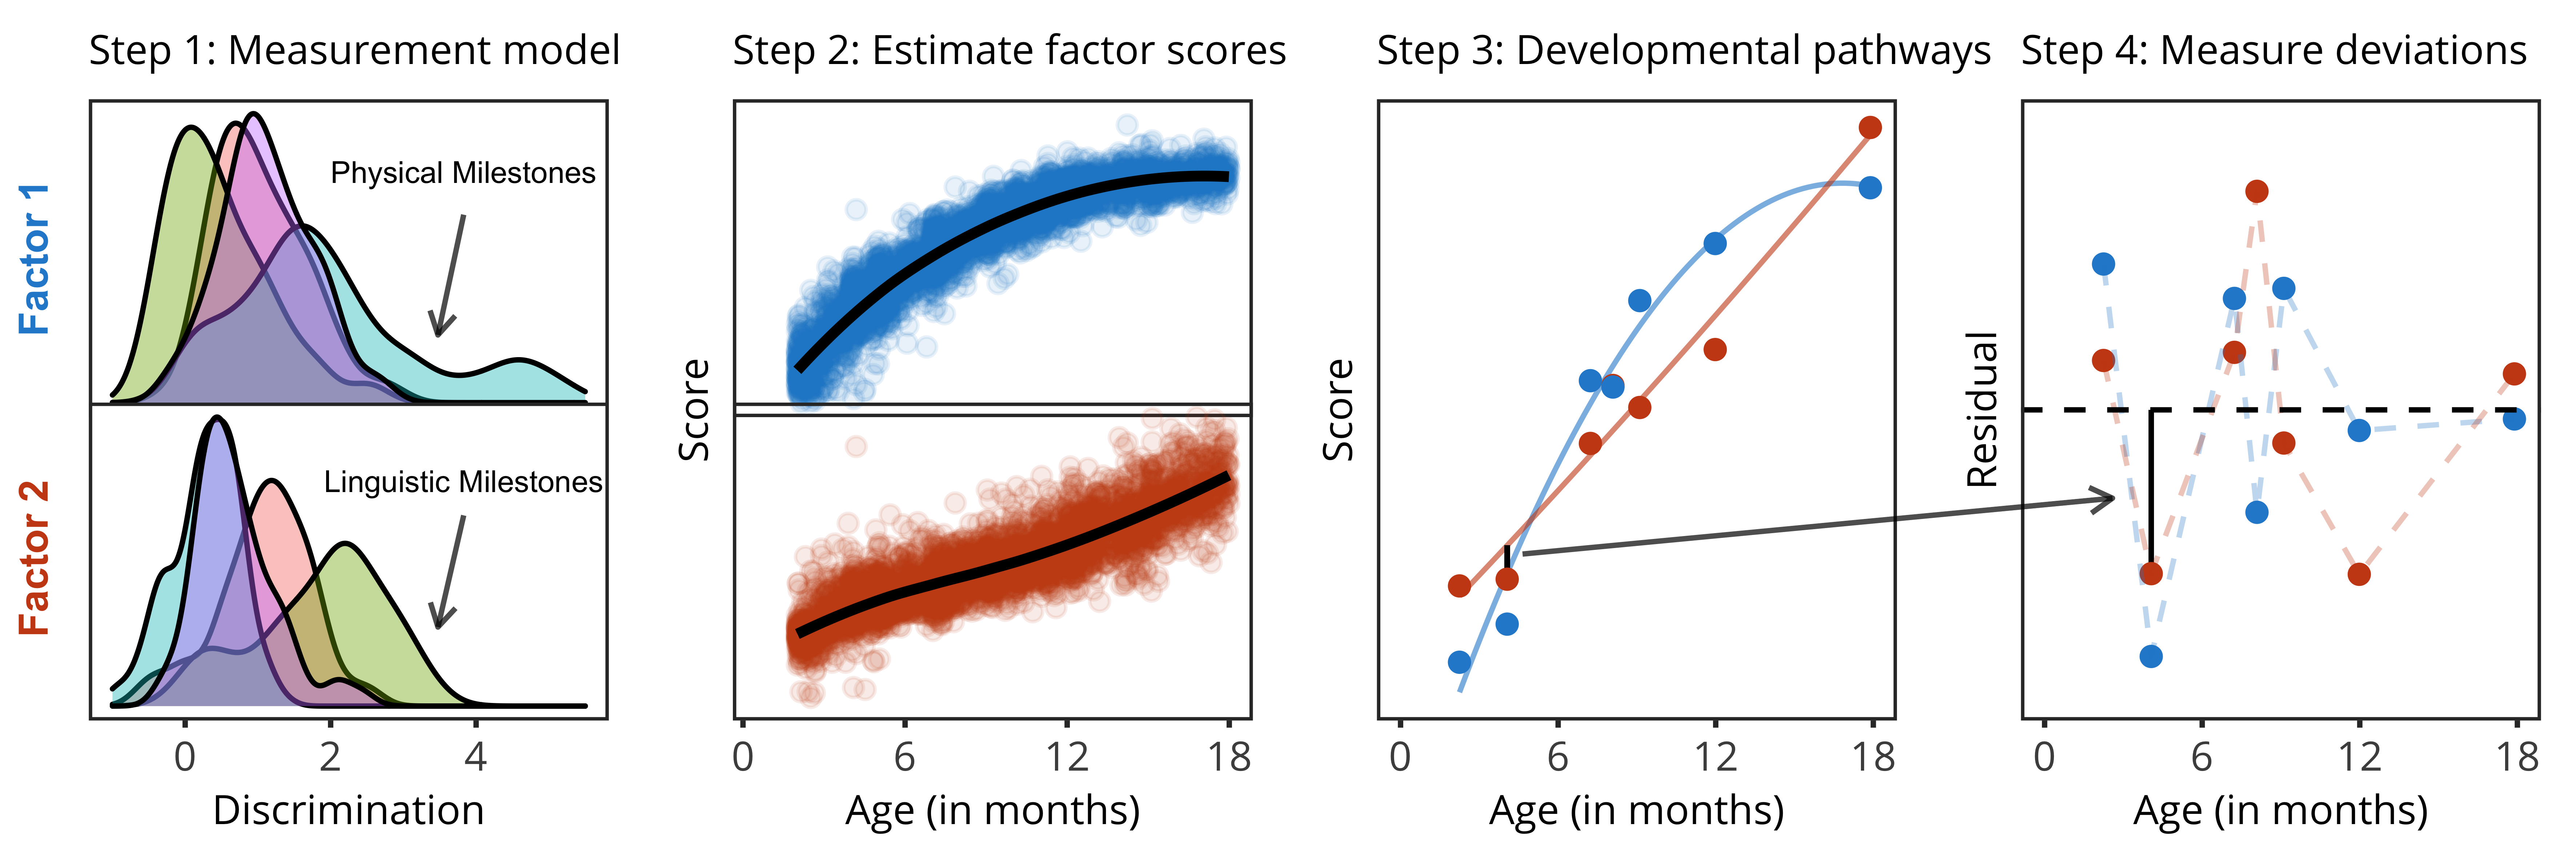
\includegraphics[width=1\columnwidth]{figures/bigfigure.png}
\caption{Each panel corresponds to a step from Study 2. In the first step, we used the survey data to develop a measurement model. The first factor is mainly physical and the second factor is mainly linguistic. In the second step, we used the measurement model to estimate factor scores for each child-timepoint in the app data. As expected, both factors are highly associated with age. In the third step, we modeled longer-term developmental trends separately for each child. Here, we illustrate this step by showing the trends for a single child. In the fourth step, we extract the deviations (i.e., residuals) from the developmental trends. Here, we show the deviations (i.e., residuals) for that same child. These deviations allow us to examine age-related differences
in within-person coupling of factor scores.}
\label{fig:study2}
\end{figure}

In all
three samples, we find strong evidence for the differentiation
hypothesis. For example, a 1-unit deviation from factor 2's
developmental pathway is associated with at least a 0.75-unit deviation
in the same direction from factor 1's developmental path at 2 months
old; and, this association decreases to less than a 0.15-unit deviation
for children older than 12 months old. We find similar results when
inverting the factors and considering the association between deviations
from factor 1's developmental pathway on deviations from factor 2's
developmental path. These results are depicted in Figure
\ref{fig:study2results}.

This finding gives strong evidence that, within individual children, local deviations from the child's own developmental growth trajectory begin quite coupled but appear to decouple by around 18 months. Put another way, when a young baby grows especially quickly or slowly they tend to do so on both relevant dimensions (at least within our milestone set).\footnote{Although models with more factors show the same differentiation effect (see Supplemental Information), the finding is easiest to conceptualize in a two-factor space.} In contrast, a toddler's language can surge forward (or hang back) without coordinated changes in motor development.
% Parallel to the cross-sectional evidence obtained in Study 1, the results from Study 2 provide evidence for the differentiation hypothesis, as a within-person process that manifests in longitudinal data.

\begin{figure}
\centering
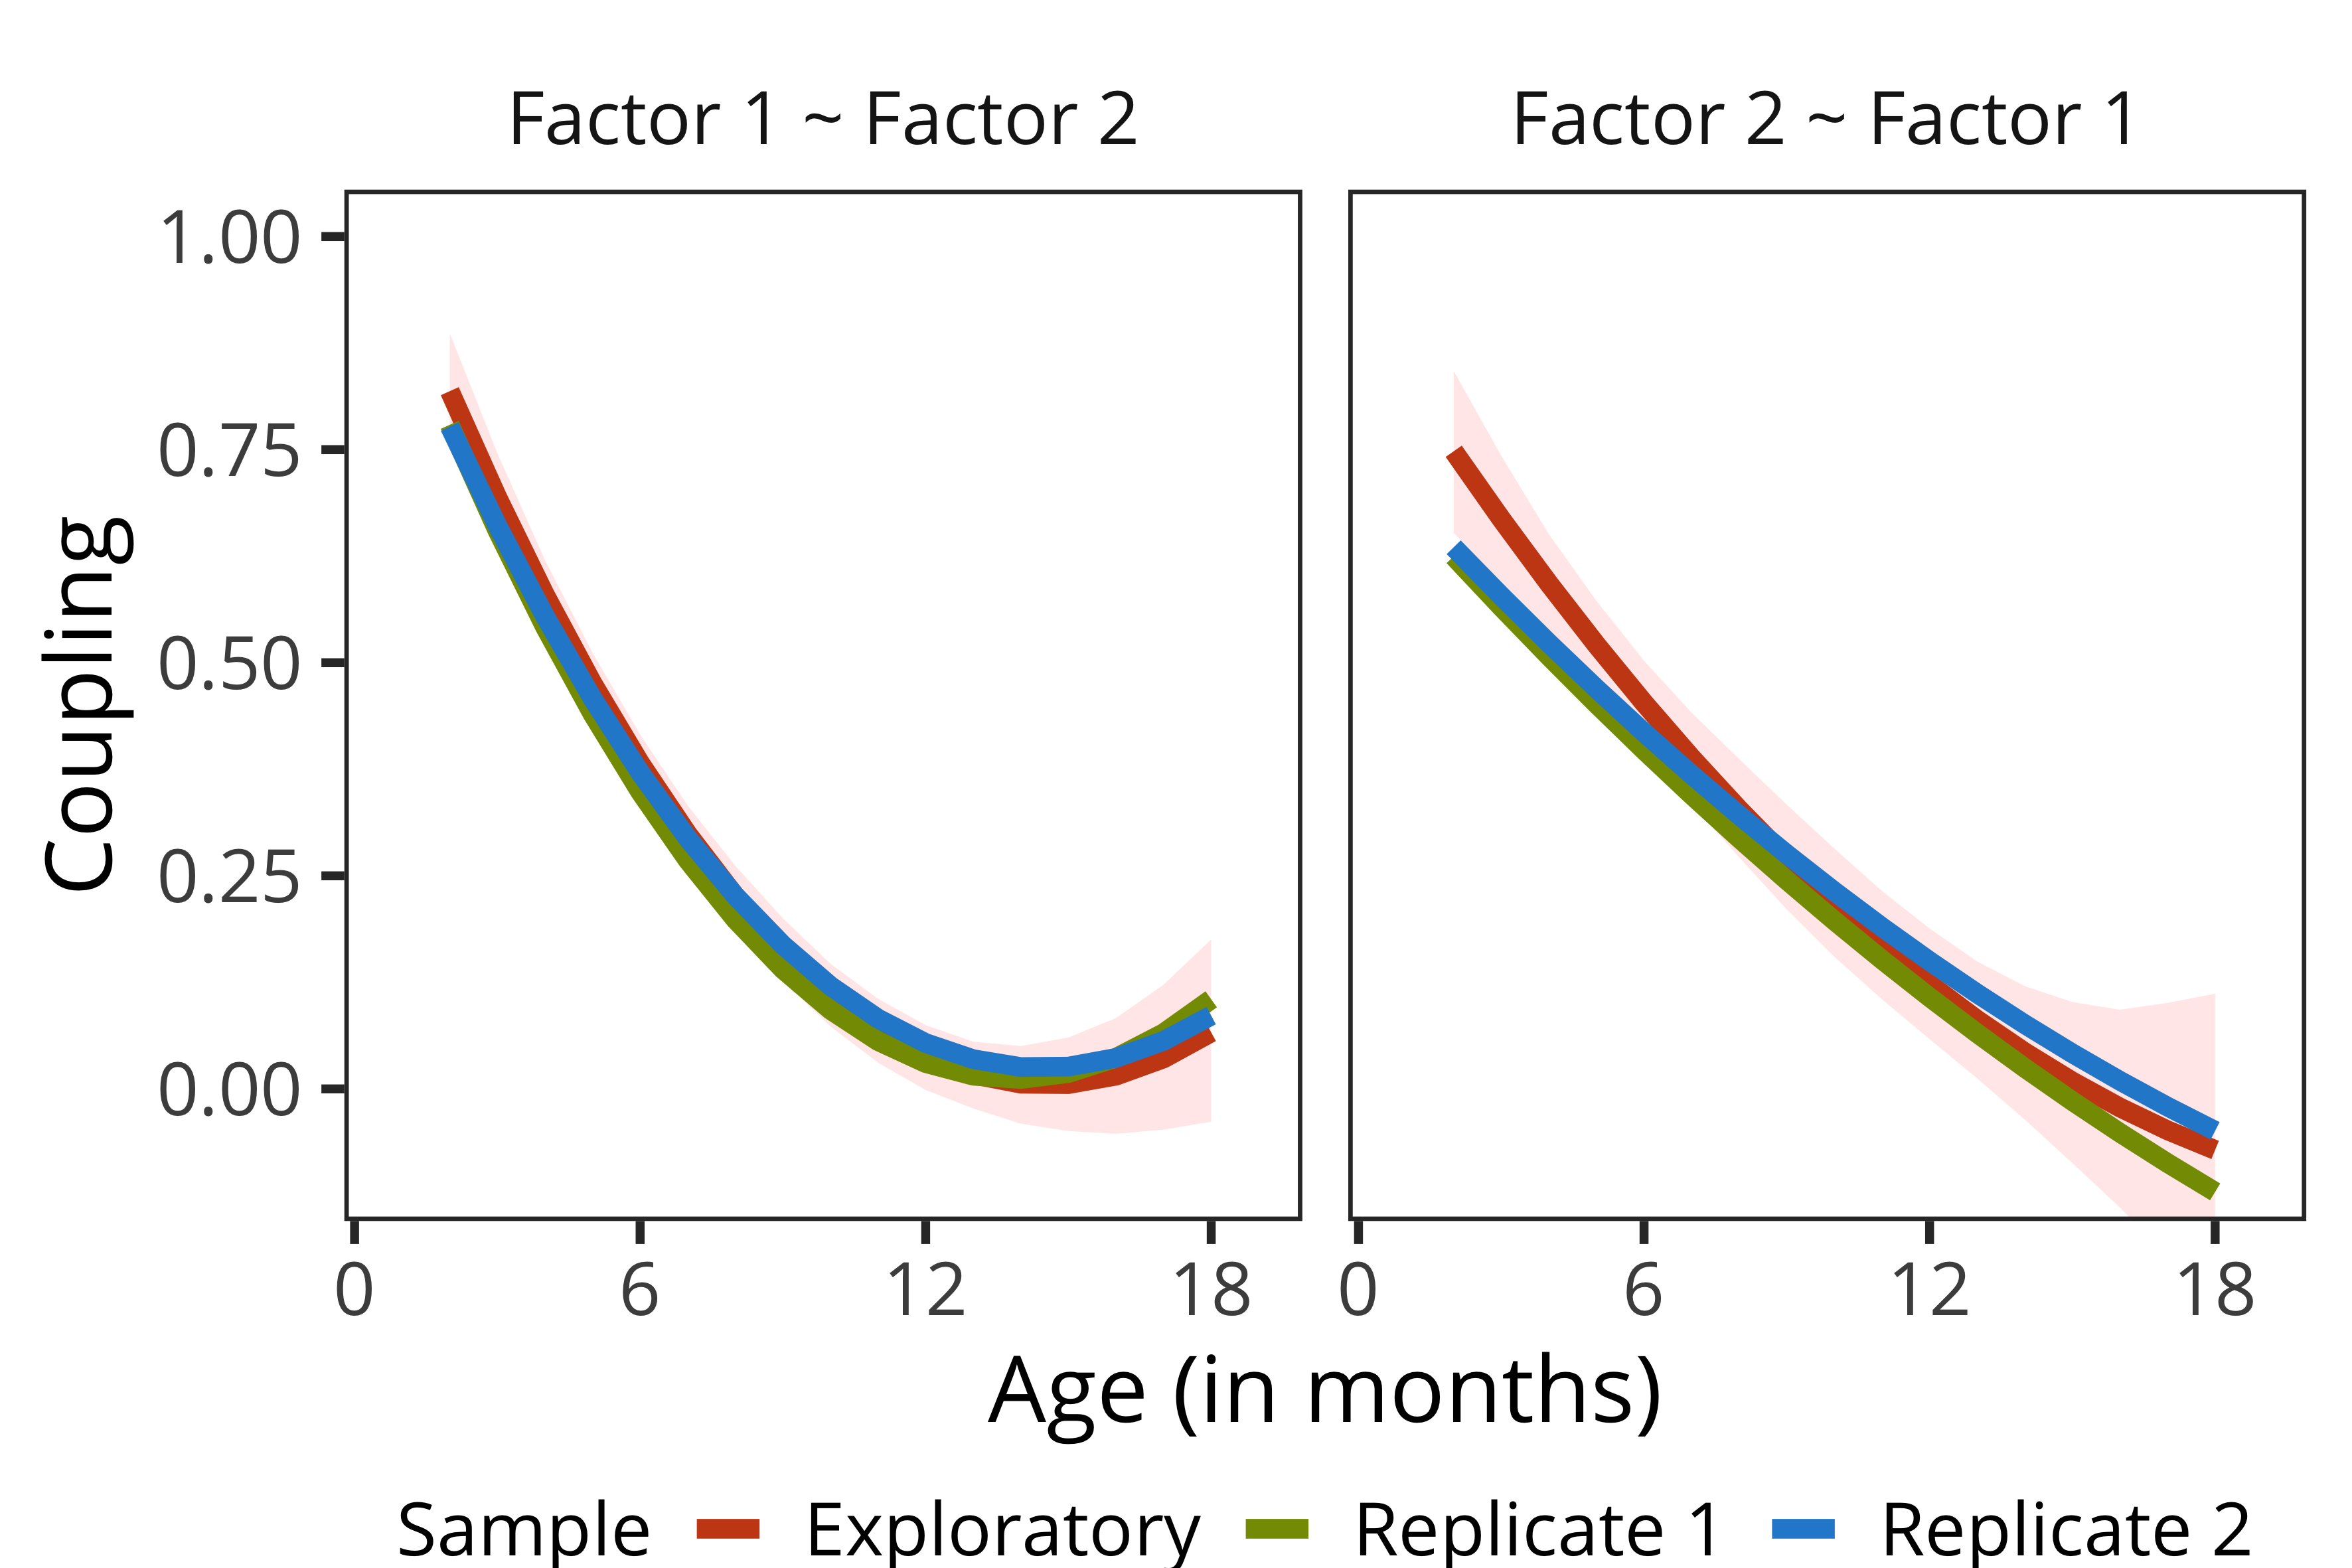
\includegraphics[width=.75\columnwidth]{figures/study2results.png}
\caption{Coupling parameters from 2 to 18 months old. Association between 1-unit deviation from the developmental pathway for one factor with deviation from the other factor’s developmental path. Left panel shows factor 1 as the dependent variable and factor 2 as the independent variable. Right panel is the inverse. As the differentiation hypothesis suggests, we find decreasing coupling over the age span. Red shading is 95\% confidence interval for exploratory sample as calculated by 1000 bootstrapped simulations.}
\label{fig:study2results}
\end{figure}

\section{General Discussion}

Is early child development a single unified process or a host of different
processes? Stage theories assume synchronization in developmental
changes across distinct domains like language, social-emotional
development, and cognition \parencite{flavell1963}. In contrast, more modern modular theories
tend to assume that particular aspects of development proceed ``on their
own schedule'' \parencite{spelke1992,sheldrick2019}. Here, inspired by psychometric studies of
age-related changes in cognition, we explored this issue through the lens of individual variation.


Our work makes three contributions.
First, we describe the between-child multidimensional structure of
developmental variation in early child. Second, we find that the
dimensionality of this variation increases with age, constituting between-person evidence for the differentiation hypothesis. Third, we find that
within-child covariation between factors decreases during a child's
first year, constituting within-person evidence for the differentiation hypothesis.
% Our premise was that
% understanding the nature of variation in developmental milestones could help shed
% light on whether children's developmental change covaries across domains
% within a single factor and whether developmental variation splits into multiple factors as children grow older.

With the emergence of data science techniques, our use of newly
available data is a specific instance of a general pattern: Larger data
enables more precise measurements, which can be used to test and refine theories.
Although many studies have assessed developmental differentiation in
to our knowledge the differentiation hypothesis has not previously been tested using large-scale
data from young children \cite{breit2021}.
Our contributions came from leveraging data made newly available
due to parents' use of a mobile app. Parents, who were looking to understand and
support their child's development, answered hundreds of binary milestone
questions about their child. As a result, we were able to explore and
test the differentiation hypothesis from birth through early childhood.
 % by fitting a
% variety of psychometric models to this data.

% What are the developmental factors that these models identified?
The dimensions of variation in development that we identified appeared to map to some extent onto classic domains of development, for example by loading more heavily on motor or language milestones.
It is important to remember, however, that by nature of our analyses, our results describe differences rather than commonalities between individuals. Because we leverage individual variability, our models are not designed to detect the operation of mechanisms that are consistent across individuals. Despite the variation we observed and quantified, many common mechanisms (from statistical learning to motor skill learning) likely support developmental change across all individuals. The individual differences in milestones that we observe then might be differences in learning rates across individuals.

One major axis of differentiation was between motor and linguistic milestones. While these two aspects of development were tightly coupled initially, they appeared to decouple over the first year and a half. This observation is interesting from the perspective of prior theories about the relationship between language and motor development. For example, \cite{iverson2010} argues for two routes of influence. First, early linguistic skills like babbling are motoric in nature and hence may be influenced by the same kinds of experiences (as well as following the same maturational timetable). This route is supported in our data. Second, motor development opens up new opportunities for learning, for example, by allowing children to locomote to new objects and bring them back to their parents. While this observation is supported in some more detailed studies \parencite[e.g.,][]{walle2014,karasik2014}, it was not borne out in the broad developmental view afforded by our data.

Our work has several limitations that should inform future work. First,
we relied on parent report, which can have significant biases and
limitations, especially in its precision regarding capacities that are
difficult to observe \parencite[e.g., cognitive abilities;][]{frank2021,feldman2000}. Second, our
data come from very specific populations (Study 1: middle- and
upper-class Mexican parents whose children were in group care; Study 2:
an unknown but largely Brazil, US, and Mexico-based group of users of a developmental mobile application) and hence
caution is warranted in generalizing to specific populations. Third, our results are with regard to child development
as defined by the Kinedu app milestone set. These milestones provide a global picture of observable developmental changes, but they do not necessarily carve development at its joints.
% Further, the factor discovery methods we use reflect the statistical structure of the observed data rather than the structure of any latent variables internal to the child \parencite{bork2017,maraun2003,van-der-maas2006}.

This study illustrates how
large datasets can be leveraged to better understand child development. By
combining multiple data sources and developing novel methods we
were able to engage new exploration and testing of long-standing theories of child development. We found evidence that children's development is better characterized as multidimensional than as unidimensional, and evidence in support of both between- and within-person versions of the
developmental differentiation hypothesis. Our hope is
that this work encourages others to continue to advance developmental
theory by taking advantage of opportunities provided by new,
larger data sources.

\printbibliography
\end{document}
